\documentclass{article}
\usepackage{pgfplots}
\pgfplotsset{compat=1.18}

\begin{document}

\begin{figure}[h]
    \centering
    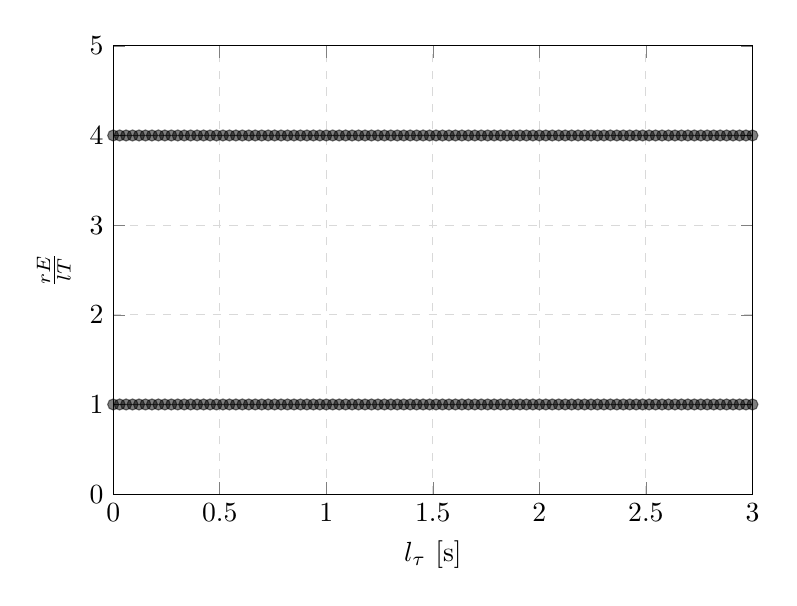
\begin{tikzpicture}
        \begin{axis}[
            xlabel={$l_{\tau}$ [s]},
            ylabel={$\frac{\prescript{r}{}{E}}{\prescript{l}{}{T}}$},
            xmin=0, xmax=3,
            ymin=0, ymax=5,
            xtick={0,0.5,...,3},
            ytick={0,1,...,5},
            width=0.8\textwidth,
            height=0.6\textwidth,
            grid=major,
            grid style={dashed, gray!30},
            every axis plot/.append style={
                mark=none,
                domain=0:3,
                samples=100,
                smooth
            },
            every axis plot post/.append style={
                mark=*
            }
        ]
            \addplot[black, fill=black, opacity=0.5] {4};
            \addplot[black, fill=black, opacity=0.5] {1};
        \end{axis}
    \end{tikzpicture}
    \caption{Coordination diagram for a deadlock situation: There is no collision-free path from start to goal in $\mathcal{C}$. The durations of the separately computed trajectories are $\prescript{r}{}{T} = 4.53$\,s and $\prescript{l}{}{T} = 2.72$\,s.}
    \label{fig:deadlock_diagram}
\end{figure}

\end{document}